\documentclass{article}\usepackage[]{graphicx}\usepackage[]{color}
% maxwidth is the original width if it is less than linewidth
% otherwise use linewidth (to make sure the graphics do not exceed the margin)
\makeatletter
\def\maxwidth{ %
  \ifdim\Gin@nat@width>\linewidth
    \linewidth
  \else
    \Gin@nat@width
  \fi
}
\makeatother

\definecolor{fgcolor}{rgb}{0.345, 0.345, 0.345}
\newcommand{\hlnum}[1]{\textcolor[rgb]{0.686,0.059,0.569}{#1}}%
\newcommand{\hlstr}[1]{\textcolor[rgb]{0.192,0.494,0.8}{#1}}%
\newcommand{\hlcom}[1]{\textcolor[rgb]{0.678,0.584,0.686}{\textit{#1}}}%
\newcommand{\hlopt}[1]{\textcolor[rgb]{0,0,0}{#1}}%
\newcommand{\hlstd}[1]{\textcolor[rgb]{0.345,0.345,0.345}{#1}}%
\newcommand{\hlkwa}[1]{\textcolor[rgb]{0.161,0.373,0.58}{\textbf{#1}}}%
\newcommand{\hlkwb}[1]{\textcolor[rgb]{0.69,0.353,0.396}{#1}}%
\newcommand{\hlkwc}[1]{\textcolor[rgb]{0.333,0.667,0.333}{#1}}%
\newcommand{\hlkwd}[1]{\textcolor[rgb]{0.737,0.353,0.396}{\textbf{#1}}}%
\let\hlipl\hlkwb

\usepackage{framed}
\makeatletter
\newenvironment{kframe}{%
 \def\at@end@of@kframe{}%
 \ifinner\ifhmode%
  \def\at@end@of@kframe{\end{minipage}}%
  \begin{minipage}{\columnwidth}%
 \fi\fi%
 \def\FrameCommand##1{\hskip\@totalleftmargin \hskip-\fboxsep
 \colorbox{shadecolor}{##1}\hskip-\fboxsep
     % There is no \\@totalrightmargin, so:
     \hskip-\linewidth \hskip-\@totalleftmargin \hskip\columnwidth}%
 \MakeFramed {\advance\hsize-\width
   \@totalleftmargin\z@ \linewidth\hsize
   \@setminipage}}%
 {\par\unskip\endMakeFramed%
 \at@end@of@kframe}
\makeatother

\definecolor{shadecolor}{rgb}{.97, .97, .97}
\definecolor{messagecolor}{rgb}{0, 0, 0}
\definecolor{warningcolor}{rgb}{1, 0, 1}
\definecolor{errorcolor}{rgb}{1, 0, 0}
\newenvironment{knitrout}{}{} % an empty environment to be redefined in TeX

\usepackage{alltt}
\IfFileExists{upquote.sty}{\usepackage{upquote}}{}
\begin{document}

\subsection{Abandon \textit{Polygonum}}
1320 seeds of each species were planted. How did it turn out?\\
% latex table generated in R 3.6.2 by xtable 1.8-4 package
% Tue Feb  2 11:06:50 2021
\begin{table}[ht]
\centering
\begin{tabular}{rrrrr}
  \hline
 & V1 & 0 & 1 & 1* \\ 
  \hline
C.canadensis & 7484 & 27551 & 578 &   0 \\ 
  H.matronalis & 7775 & 26639 & 1280 &   0 \\ 
  P.virginiana & 7893 & 27638 &  88 &  21 \\ 
   \hline
\end{tabular}
\end{table}


 That means the overall germination rate for \textit{P. virginiatum} is 6\%. I don't think any real analysis is possible with this, especially because that is across all treatment combinations.\\
\subsection{Cryptic \textit{Cryptotaenia}}
What about the germination percentages of the \textit{C. canadensis} and \textit{H. matronalis} trials across stratification treatment?
% latex table generated in R 3.6.2 by xtable 1.8-4 package
% Tue Feb  2 11:06:50 2021
\begin{table}[ht]
\centering
\begin{tabular}{rrr}
  \hline
 & C.canadensis & H.matronalis \\ 
  \hline
6 &  58 & 317 \\ 
  12 & 223 & 323 \\ 
   \hline
\end{tabular}
\end{table}

Bad germination for \textit{C. canadensis} in the 6 week stratification treatment, but maybe this can be a density effect in a model?\\

Now, what about temporal effects?

     0      1 
105001   1946 
% latex table generated in R 3.6.2 by xtable 1.8-4 package
% Tue Feb  2 11:06:51 2021
\begin{table}[ht]
\centering
\begin{tabular}{rlrrr}
  \hline
 & taxa & strat & mean.time & sd.time \\ 
  \hline
1 & C.canadensis &   6 & 7.90 & 2.01 \\ 
  2 & C.canadensis &  12 & 5.33 & 2.30 \\ 
  3 & H.matronalis &   6 & 2.94 & 1.73 \\ 
  4 & H.matronalis &  12 & 2.06 & 0.92 \\ 
   \hline
\end{tabular}
\end{table}

 The shift in temporal offset (priority effect) is only a mean of 1.9 days with high SD. This I think is because of the strong co-variance between germination percentage and timing in this current trial.\\
 
 So upshot: Maybe you can still answer a very applied question about biological and environmental factors influence Cc competing with Hm?\\
 
 germperc_{(0,1)} \ = planted_{con-specific} $+$ planted_{competitor} $+$ stratification\\

 growthrate \ = planted_{con-specific} $+$ planted_{competitor} $+$ stratification\\
 
 Are there enough seeds for 2 harvests?\\
% latex table generated in R 3.6.2 by xtable 1.8-4 package
% Tue Feb  2 11:06:51 2021
\begin{table}[ht]
\centering
\begin{tabular}{rrllr}
  \hline
 & strat & taxa & harvest & n \\ 
  \hline
1 &   6 & C.canadensis & early & 36.00 \\ 
  2 &   6 & C.canadensis & late & 22.00 \\ 
  3 &   6 & H.matronalis & early & 159.00 \\ 
  4 &   6 & H.matronalis & late & 158.00 \\ 
  5 &  12 & C.canadensis & early & 105.00 \\ 
  6 &  12 & C.canadensis & late & 118.00 \\ 
  7 &  12 & H.matronalis & early & 161.00 \\ 
  8 &  12 & H.matronalis & late & 162.00 \\ 
   \hline
\end{tabular}
\end{table}

Also, should I keep the CC and Hm monocultures from Pv trials to bring more data in?\\ 
\subsection{OR: To the Autoclave they go...}

Basically, I am not sure what this experiment would add to the literature consider there have already been simular papers on Hesperis published...see attached to email.\\


\subsection{A purpose for a pilot}
A concept paper: Testing seasonal priority effects in temperate environments (ie seed w/ dormancy) would require some minimum amount of inter-specific variation in temperature sensitivity. A major question is does this variation exist at levels high enough to match the planting intervals that generate priority effect. Luckily, two recent papers in Restoration ecology have reviewed these studies. I could:\\
\begin{enumerate}
\item Revisit these review the quantify the minimum sowing interval that still produce priority effects
\item See what sort of chilling differences are needed to reproduce these differentials (based on pilot, see plot below)
\item Compare to interannual variation in stratification or climate change projections.
\end{enumerate}

\begin{figure}[h!]
        \centering
         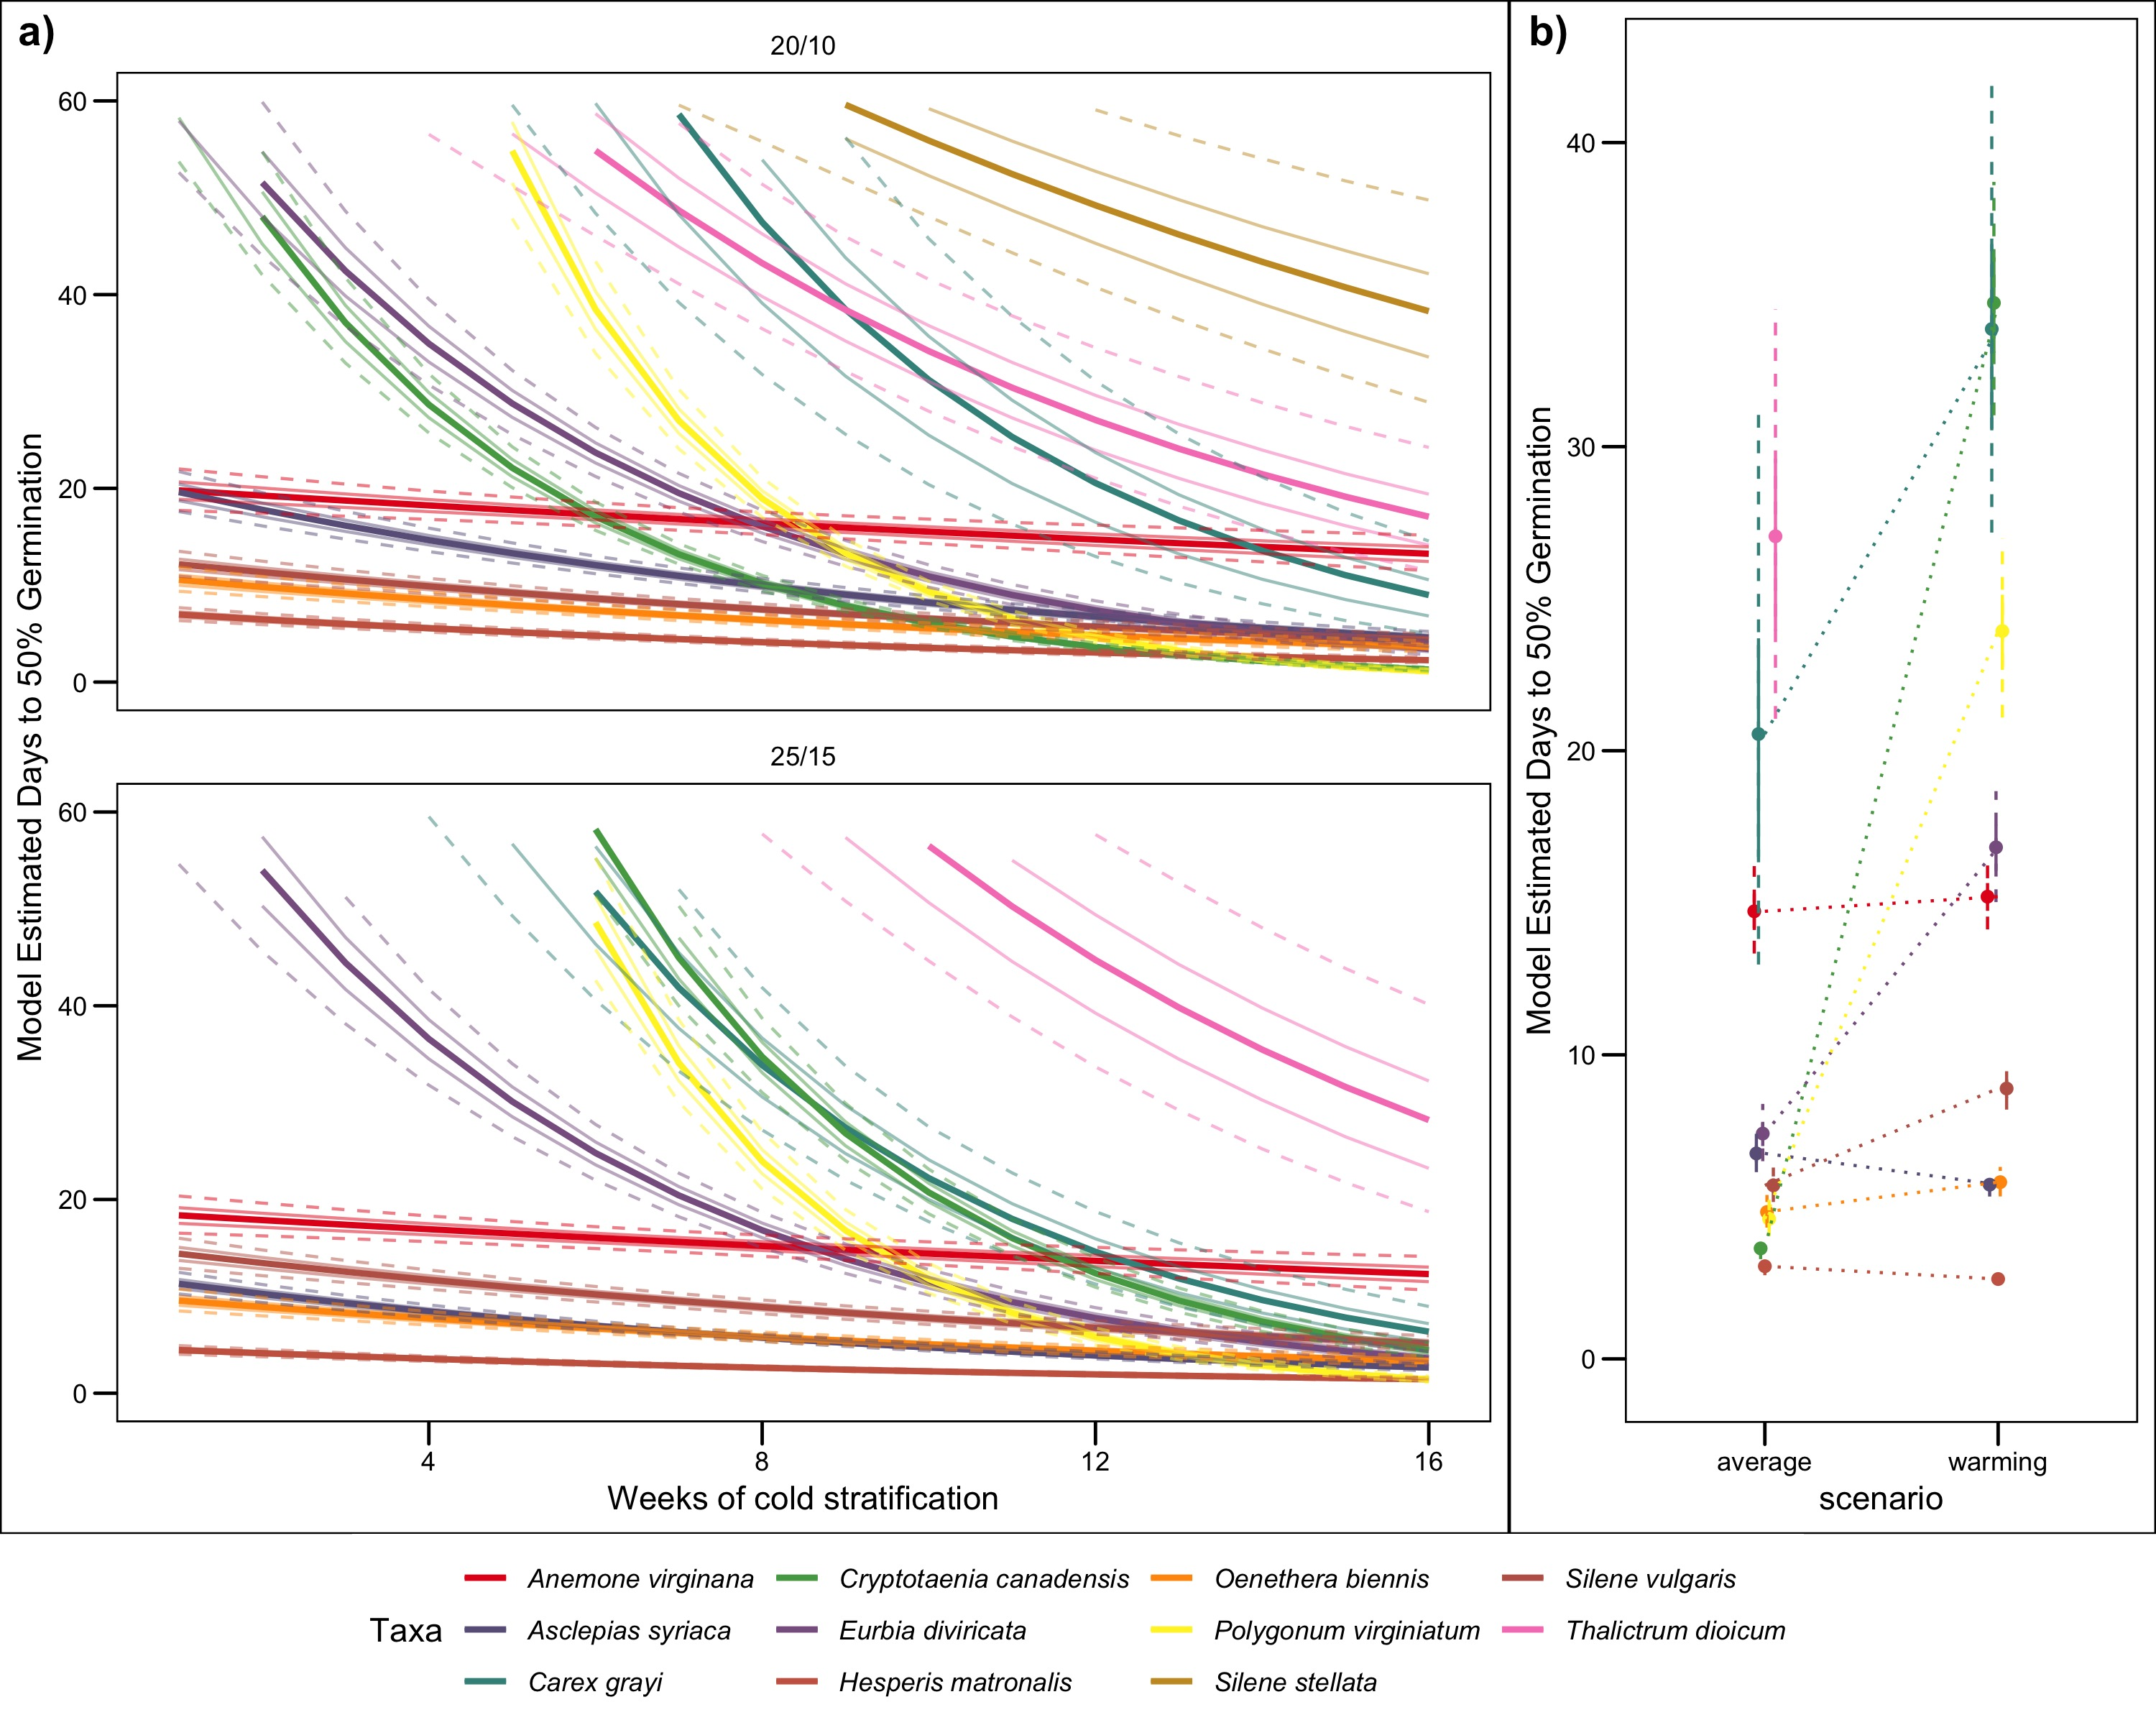
\includegraphics[width=\textwidth]{../figure/AFTplots.jpeg}
                 \caption{Accelerate failure time models for mean germination time for my pilot study at different stratification duration.}
    \end{figure} 

\end{document}
